\chapter{Desenvolvimento}\label{cap2}
 Nessa seção será apresentado o escopo do projeto e a proposta de solução.
\section{Escopo}
Para definição do escopo do projeto foram analisados os seguintes aspectos: Local de atuação, localização da apoio, situações de socorro pré-hospitalar, viabilidade dos itens a serem levados pelo VANT, elementos estruturais e planejamento de atuação e estratégia de voo do VANT e o método de comunicação com o usuário.
\begin{description}
  \item[Local de Atuação] \hfill 
  	\begin{itemize}
  		\item Locais de difícil acesso no DF seja por natureza ou circunstância e será acionado apenas quando houver necessidade.

  	\end{itemize}
  \item[Tipo de emergência] \hfill 
  	\begin{itemize}
  		\item Paradas/Ataques Cardíacos;
		\item Paradas Respiratórias;
		\item Hemorragias Externas.
  	\end{itemize}
  \item[Equipamentos Utilizados para salvamento] \hfill \\
  	Para definir os itens a serem levados foi realizada uma análise de viabilidade levando em consideração a utilização dos equipamentos por pessoas sem conhecimento em salvamento e a possibilidade de carga útil do VANT.
  	\begin{itemize}
  		\item Kit primeiro socorros;
		\item Desfibrilador Automático;
		\item Reanimador ventilatório manual;
		\item Kit para hemorragias externas.
  	\end{itemize}
  \item[Distância de Operação] \hfill 
  	\begin{itemize}
  		\item Haverá uma única central de controle;
  		\item Velocidade máxima do drone: 70 km/h;
  		\item O VANT operará em um raio de 20 km. Sendo que o centro do raio é a ambulância, que vai ser de onde o VANT irá partir.
  	\end{itemize}
  \item[Sinais vitais que serão monitorados] \hfill 
  	\begin{itemize}
  		\item Eletrocardiograma.
  	\end{itemize}
  \item[Projeto mecânico estrutural] \hfill 
  	\begin{itemize}
  		\item Asa rotatória;
		\item Elétrico.
  	\end{itemize}
  \item[Materiais] \hfill 
  	\begin{itemize}
  		\item Polímeros compostos;
		\item Fibra de carbono.
  	\end{itemize}
  \item[Controle] \hfill 
  	\begin{itemize}
  		\item Controle automático comandado pela central de comunicação. (Rádio frequência).
  	\end{itemize}
  \item[Comunicação entre equipe de paramédicos e usuário] \hfill 
  	\begin{itemize}
  		\item Câmera e sistema de áudio. Sendo que, o vídeo será apenas para o paramédico da central e a comunicação via áudio para ambos;
  		\item O usuário apenas escutará as instruções, comunicando-se apenas através do áudio.
  	\end{itemize}
  \item[Sensores] \hfill 
  	\begin{itemize}
  		\item Eletrocardiograma para medir os sinais vitais;
		\item GPS (u-blox LEA-6H.)- Utilizado para o deslocamento e localização do VANT;
		\item Acelerômetro e Magnetometro (ST Micro LSM303D) - Utilizado para obter uma localização mais apurada;
		\item Giroscópio (ST Micro L3GD20) - Refinamento na localização;
		\item Controladora Pixhawk (PX4).
  	\end{itemize}
  \item[Projeto unidade central de processamento] \hfill 
  	\begin{itemize}
  		\item Controladora Pixhawk (PX4).
  	\end{itemize}
  \item[Conversão e armazenamento de energia] \hfill 
  	\begin{itemize}
  		\item Bateria de polímeros de Lítio (LiPo).
  	\end{itemize}
  \item[Estimação de consumo energético e autonomia] \hfill 
  	\begin{itemize}
  		\item 50 minutos de voo
  	\end{itemize}
\end{description}

\section{Estrutura Analítica de Projeto - EAP}

No desenvolvimento de qualquer projeto, é essencial ter uma visão geral sobre as atividades que serão realizadas no decorrer da processo de criação.  Para isso existem formas de sistematização e organização dessas informações.

Uma dessas formas de organizar a informação é a EAP - Estrutra Analítica do Projeto - que é a estruturação das entregas a serem completadas em forma de árvore de maneira hierárquica, onde são distribuídas da mais gerais para as mais especificas.

A EAP foi a forma escolhida pela equipe de desenvolvimento do projeto EmerVant para estruturação das entregas, por proporcionar de uma maneira simples e objetiva todos os pontos abordados e discutidos para a realização do projeto em seu devidos graus de importância. 

Para a criação da EAP do EmerVant, foi observado que dentro do projeto há varias áreas de atuação. Assim os níveis mais gerais foram definidos por essas áreas de atuação que são:
\begin{itemize}
\item Gerência de Projetos;
\item Iniciação;
\item Estrutura do VANT;
\item Comunicação;
\item Controle;
\item Fonte Energética;
\item Encerramento.
\end{itemize}

\begin{figure}[ht]
  \centering
    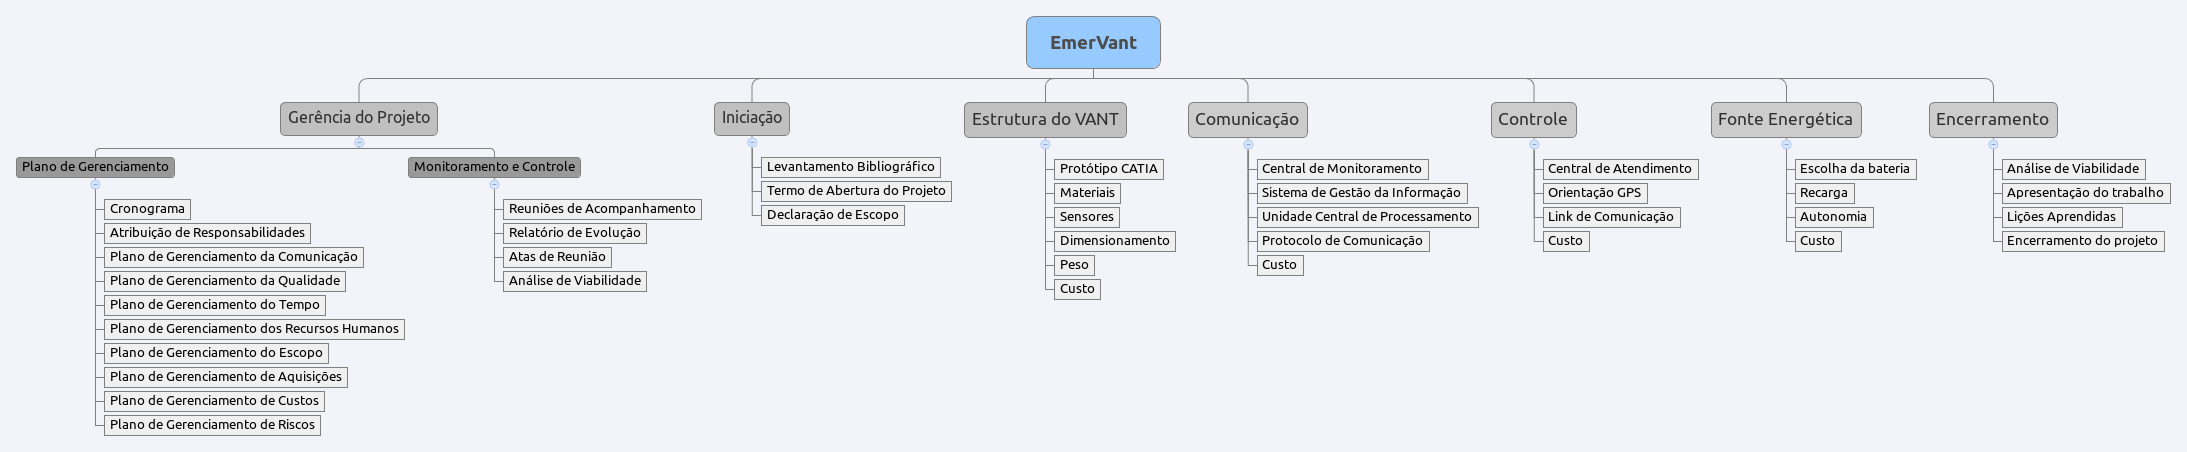
\includegraphics[keepaspectratio=true,scale=0.7,angle=90]{figuras/eap.eps}
  \caption{Estrutura Analítica do Projeto EmerVant}
\end{figure}

As entregas especificas de cada tópico foram baseadas nas definições de escopo e requisitos. A Figura 5 é a representação gráfica da EAP criada para o projeto EmerVant.

\section{Solução Inicial}

  O EmerVant consiste em um sistema de assistência emergencial através da utilização de um VANT.	

O grande potencial dos drones tem sido explorado em inúmeras implementações militares e civis. Entre os vários VANTs, estes de pequena escala são atraentes para o meio acadêmico, devido ao seu pequeno tamanho, as capacidades de voo único, excelente dirigibilidade e baixo custo. \cite{SDM}.

O VANT escolhido para a aplicação foi o multirotor de oito hélices, conhecido como octocóptero. Usando um essa configuração a força de sustentação é melhor dividida entre os múltiplos motores possibilitando carregar uma maior carga útil e tendo uma maior estabilidade.

O \textit{Global Position System} (GPS) é o sensor de maior importância deste projeto, pois as informações fornecidas serialmente por esse componente auxiliam não só na estabilização da aeronave mas no controle e na locomoção do VANT até o local desejado.

Em uma situação normal o desempenho do piloto automático excede a que é controlada por humanos, e mesmo em situações mais desafiadoras sua performance é equivalente.

O projeto mecânico estrutural será constituído de polímeros compostos e fibra de carbono. O VANT será de asa rotativa e utilizará alguns sensores que serão processados por sistemas embarcados dedicados ao voo. 

O controle será feito através de um sistema automático com o uso de GPS, utilizado para deslocamento e localização. Através desse sensor o piloto automático tem acesso às informações em tempo real, utilizando-as ele consegue guiar-se, dessa maneira ele sabe exatamente seu lugar no espaço e sua localização à obstáculos. Para gerar essas informações são necessários: giroscópios, acelerômetro, sensores magnéticos e eletromagnéticos, sensores visuais, sensores ultrassom, infravermelhos, micro-ondas e gamas de rádio. \cite{UDE}

Seu local de atuação será na Esplanada dos Ministérios. Quando acionado a central, que fica em um ponto estratégico da Esplanada, irá receberá a informação referente a necessidade e irá passar de forma serial para o drone as coordenadas referentes  ao local e situação da(s) vítima(s).

O monitoramento do VANT ocorrerá através de um sistema de controle automático por rádio frequência que será monitorado e comandado pela central de monitoramento. Ele terá uma câmera e um sistema de áudio.

O VANT, através da câmera e do sistema de áudio estabelecerá a comunicação entre o usuário,a ambulância e a central de monitoramento. O vídeo será apresentado apenas para o paramédico da central e o áudio para a central e a ambulância. O contato do usuário será apenas com o áudio.

O paramédico dará orientações para quem está com a vítima através do sistema de comunicação do EmerVant. Com a câmera os paramédicos da central de comando poderá visualizar a situação, dar instruções para utilizar o desfibrilador ou reanimador ventilatório manual. 


\section{Cronograma}
O cronograma preliminar das atividades pode ser visto na Figura 6, e o gráfico de Gantt que relaciona as tarefas com o tempo está representado na Figura 7. As atividades estão mais especificadas apenas no Ponto de Controle 1, os demais pontos de controle estão planejados de forma macro.

 \begin{figure}[ht]
	\centering
		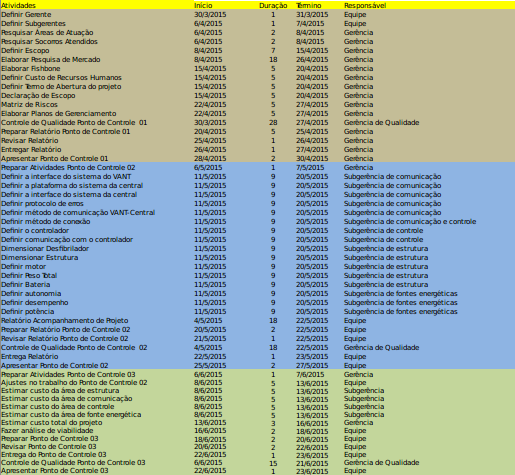
\includegraphics[keepaspectratio=true,scale=0.9]{figuras/cronograma.eps}
	\caption{Cronograma de Atividades}
\end{figure}

 \begin{figure}[ht]
	\centering
		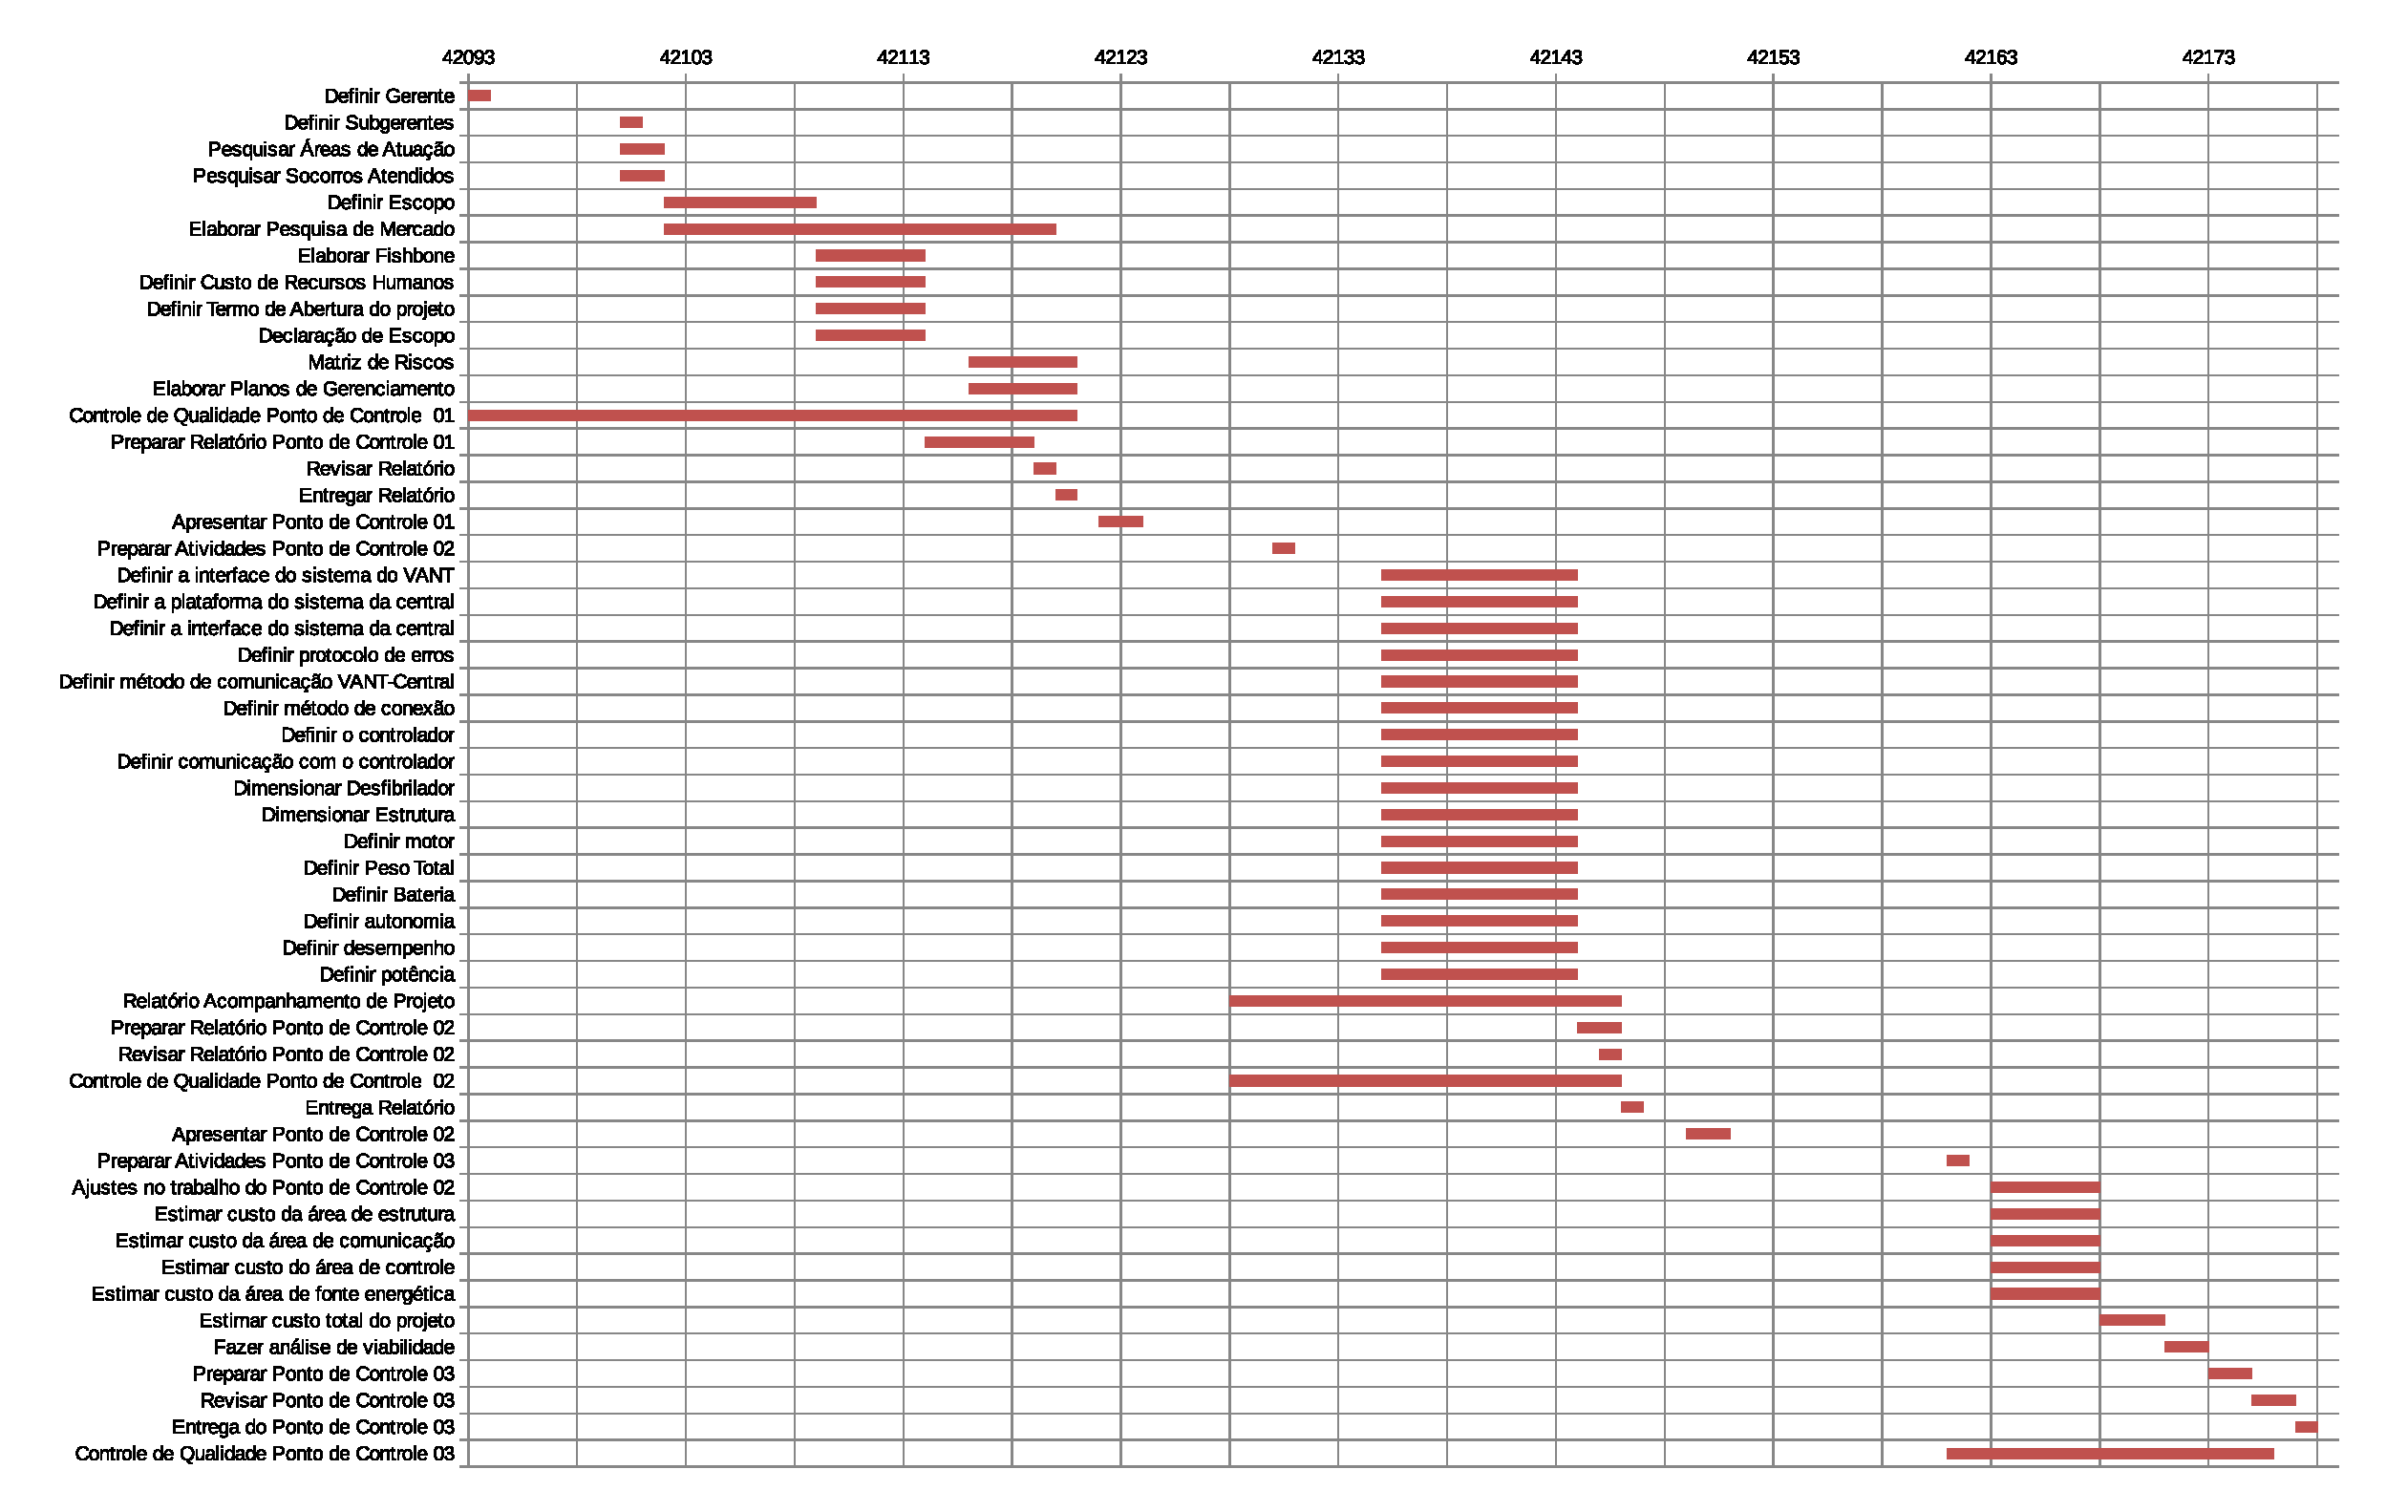
\includegraphics[keepaspectratio=true,scale=0.9,angle=90]{figuras/gantt.eps}
	\caption{Gráfico de Gantt}
\end{figure}


